\section{Architecture Overview}
\label{section:architecture_overview}

The model presented in Figure~\ref{fig:model} organises all the components involved in this system and their communications.
It considers a scenario where an embodied agent plays a physical card game against human players over a touch table.

\begin{figure}[ht]
  \centering
    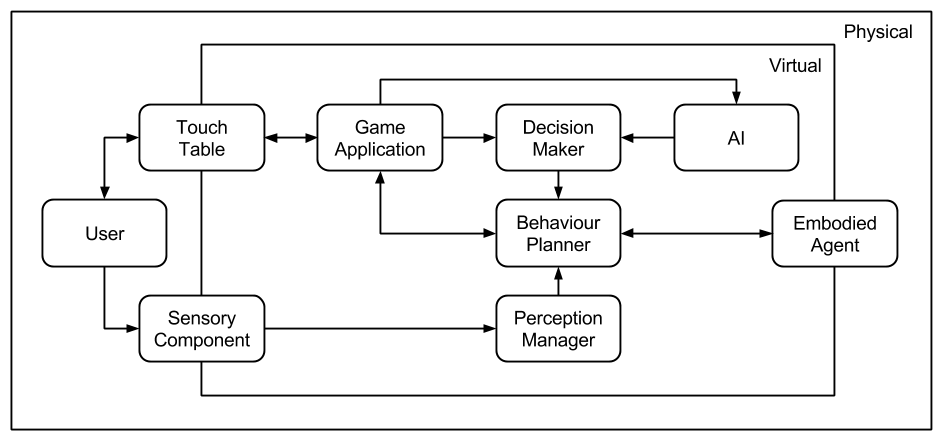
\includegraphics[width=1\textwidth]{./img/architecture}
  \caption{System architecture using components}
\label{fig:architecture}
\end{figure}

First of all, this model distinguishes physical components from virtual ones.
However, some entities are presented as both physical and virtual components and will not be detailed since their usage in this system did not demand any extensions for the scope of our domain (\emph{Touch Table}, \emph{Sensory Component} and \emph{Embodied Agent}).

The basic work-flow that illustrates the main functionalities of each component is as follows.
The human players, \emph{Users}, play with physical cards on top of a \emph{Touch Table}, and their game actions are managed by the \emph{Game Application} and communicated to both the \emph{\ac{ai}} and the \emph{Decision Maker}.
\todo[inline]{check the sensory components!}
Besides their game actions, \emph{Users} also produce another sort of events that are captured by the \emph{Sensory Component} and handled by the \emph{Perception Manager}, for instance, face movements or the source direction of spoken interactions.
The \emph{\ac{ai}} includes all the reasoning about the game and decides the next move of the artificial player.
However, the \emph{Embodied Agent} will not only play a certain card, but will also include social behaviours.
As a result, the \emph{Decision Maker} balances the \emph{\ac{ai}} decisions and game information to produce an appropriate sequence of behaviours and inform them to \emph{Behaviour Planner}.
Lastly, the \emph{Behaviour Planner}, after receiving high-level intention-directed instructions, builds a suitable plan to execute the chosen instructions, considering the state of the \emph{Embodied Agent}, information from \emph{Perception Manager}, and additional game information from the \emph{Game Application}.

\begin{figure}[ht]
  \centering
    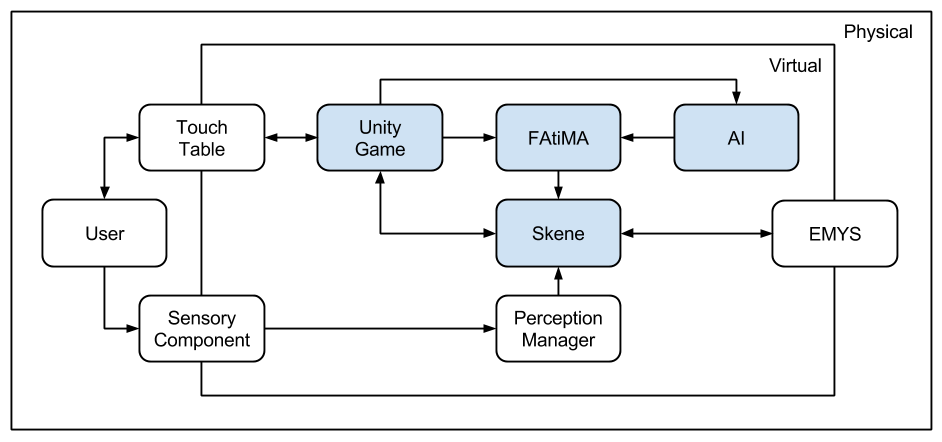
\includegraphics[width=1\textwidth]{./img/model}
  \caption{System architecture using modules}
\label{fig:model}
\end{figure}

\todo[inline]{confirmar com o Tiago se sai uma seta do skene para o unity!!!}
The previously described architecture is instantiated as shown in Figure~\ref{fig:model} and the blue modules are thalamus communicating entities.
This concept arises from the Thalamus Framework \cite{Ribeiro}, which enables the usage of entities that can be registered at runtime in a server in order to send and receive specific messages.
These entities are publishers and subscribers of the channels they want to write on and listen to, respectively.
The implementation provided by this framework works by simply inherit from the \emph{ThalamusClient} class and implement the interfaces of the messages that the entity wants to exchange.

The \emph{Unity Game} module is responsible for displaying the interface of the game, reading the physical cards, publishing all the relevant game events and subscribing to the plays of artificial players.

The chosen \emph{Behaviour Planner} is \emph{Skene} \cite{Ribeiroa}, which tightens the communication between the world and an embodied agent with a high-level behaviour description language, also known as utterances.
These utterances might include instructions for gazing, pointing, animating or sound, among other things.
Additionally, considering some instructions require target positions or other game information, Skene subscribes to \emph{Unity game} messages to keep that information updated.

The \emph{\ac{ai}} and \emph{FAtiMA} modules answer to our primary goals, for that reason, their implementations are carefully detailed in Section~\ref{sec:artificial_player} and Section~\ref{sec:behaviour_planner}, respectively.
